\documentclass[12pt]{article}
\usepackage{graphicx}

\usepackage{algorithm}
\usepackage{algpseudocode}

\usepackage[margin=1.25in]{geometry}
\usepackage{listings}
\linespread{1.5}

\title{Rendering Computer Animated Films on 
Fully Homomorphic Encrypted Data\\
6.UAP Final Report
}

\author{
Naim J. Lujan\\
naim@mit.edu\\
Supervisor: Fredo Durand\\
Department of Electrical Engineering and Computer Science
}
\date{\today}

\begin{document}
\maketitle

\section{Introduction}

The process of rendering computer animated films is computationally expensive given the complex variety of physical processes being simulated. To render a film, animation studios need to have dedicated render farms consisting of a large array of powerful computers whose sole task is to render each frame of the film. As a result of the significant amount of computing resources as well as the constant maintenance and update these rendering farms require, they are very expensive. Large studios such as Pixar have the resources to have their own rendering farms, but smaller studios need to turn to outside cloud computing to render their animated movies. Cloud computing services allow you to only pay for the compute power you need as you need it, making rendering more affordable. 

The problem with using cloud computing services is that studios are very secretive; they don't want the service to be able to see any information of their upcoming movie. Popular cloud services such as Pixar's RenderMan, Amazon EC2, Microsoft Azure, and Google Cloud promise top security of data on their service. However once data is sent to cloud services, it is vulnerable and total privacy can't be ensured. Studios want to be absolutely sure that the data they send to outside sources is rendered and completely private without solely relying on the service's security measures. I believe that the solution to this problem is to utilize a type of encryption scheme called homomorphic encryption. Using homomorphic encryption, specific types of computations can be carried out on ciphertext, and generate an encrypted result. This result, when decrypted, matches the result of operations performed on the plaintext. This allows for the sending of data across different services without exposing the data to each of those services. In theory, this would allow an animation studio to send their encrypted data to be rendered by a cloud service; when sent back, the studio can decrypt the result and obtain their rendered film ensuring that their film remains secret throughout. 

There have been several different homomorphic schemes in recent years but in this paper I will explore a promising C++ library called HElib which is an implementation of the Brakerski-Gentry-Vaikuntanathan homomorphic scheme. I will describe a basic rendering method called triangle rasterization and my implementation of this method with the use of HElib to form a proof of concept of rendering on encrypted data. Finally, I will analyze my implementation and impact it has on this problem, as well as propose future work.






\section{Homomorphic Encryption}

Homomorphic encryption allows computations to be performed on encrypted data without needing to decrypt it. Given the operation $f$ and the plaintext $p$, $decrypt(f(encrypt(p)))$ = $f(p)$. Thus, after encrypting sensitive information using this scheme, you can perform operations on the data while keeping it secure. There are several encryption schemes that are partially homomorphic, meaning that not all operations can be performed on it. For example, unpadded RSA only has homomorphic multiplication where given messages $p_{1}$ and $p_{2}$, $encrypt(p_{1}) * encrypt(p{2}) = encrypt(p_{1} * p_{2})$. Similarly Benaloh and ElGamal encryption schemes allow single homomorphic additions and multiplications respectively. For the the purpose of rendering data, we need a more powerful homomorphic encryption scheme which supports arbitrary computations. Fortunately, there are a few cryptosystems that have come out in recent years that do just that called fully homomorphic encryption schemes. The first plausible construction of a fully homomorphic encryption scheme came in 2009 from Craig Gentry and since then several others have been created. Additionally, there has been the release of a few implementations of fully homomorphic schemes. One of those is HElib, which is a C++ software library that implements the Brakerski-Gentry-Vaikuntanathan encryption scheme. In this paper, I will focus on this specific implementation as it allows arbitrary addition, subtraction, and multiplication operations to be performed homomorphically. 

Even now, fully homomorphic encryption schemes are not always practical because they require too much time to encrypt and perform homomorphic operations. A number of optimizations of the BGV scheme were given recently, which bring the overhead down to polylogarithmic. Nevertheless, there is much promise in this field and improvements are constantly being created. 

I will not focus on the practicality of using HElib, but rather on creating a proof of concept of rendering data using this encryption scheme to guarantee ultimate security. I want to show that computing securely on the cloud is possible through homomorphic encryption, even though it still may not be practical. 



\subsection{HElib (Brakerski-Gentry-Vaikuntanathan scheme)}

The HElib C++ software library is an implementation of the Brakerski-Gentry-Vaikuntanathan(BGV) homomorphic encryption scheme. This scheme is based on the learning with error (LWE) that have $2^{\lambda}$ security on known attacks where $\lambda$ is the security parameter.

To get an idea of the basic concept of the learning with error encryption, let's look at the more basic encryption scheme $C * v = \mu * v$  mod $q$ where $\mu$ is with the message as an eigenvalue, $v$ is the secret key as an eigenvector, and $C$ is the ciphertext in the form of a matrix. This scheme has additive and multiplicative homomorphic qualities as you can see with the following: $C_{1} * C_{2} * v = \mu_{1} * \mu_{2} * v$ mod $q$, and $(C_{1}+C_{2}) * v = (\mu_{1} + \mu_{2}) * v$  mod $q$.

However, this can be easily attacked by using any valid ciphertext $C$ and simply finding the $v$ among its eigenvectors. Then through solving a linear system, the message $\mu$ can be found. Fortunately, this encryption scheme can be made exponentially more difficult to crack by simply adding a and noise vector $e$ with small coefficients $(<<q)$. This results in the learning with error encryption $C * v = \mu * v + e$ mod $q$ where now $v$ is an approximate eigenvector. Adding this noise vector makes this encryption exponentially more secure but still preserves all the homomorphic capabilities when observing that $(C_{1}+C_{2}) * v = (\mu_{1} + \mu_{2}) * v + (e_{1} + e_{2})$  mod $q$ and ($C_{1} * C_{2}$ mod $q) * v = \mu_{1} * \mu_{2} * v + (\mu_{2} * e_{1} + C_{1} * e_{2})$ mod $q$.

As more computations are made homomorphically, the error grows and can eventually make the result unable to be decrypted. To solve this problem, HElib has a recrypt procedure that essentially "refreshes" the ciphertext periodically whenever the noise grows too large. This makes it possible to compute arbitrary number of additions and multiplications without increasing the noise too much.

HElib is a powerful library because it allows you to add, subtract, and multiply ciphertexts homomorphically. It uses a SIMD-like optimization known as ciphertext packing. Thus, each ciphertext is essentially a vector of encrypted plaintext integrals. Your data must be in the form of a vector before encrypting it. When you perform an operation on two ciphertext, it performs this element-wise for both vectors. As a result of its structure, this scheme is particularly effective with problems that can benefit from some level of parallel computation. 

To get an idea of its performance, below is a table showing the timing of addition and multiplication I calculated, which varies by level, security, and plaintext characteristics such as word size. As you can see, multiplication takes a lot longer than addition because it increases the noise at a much larger rate as seen with the equations above. This requires more noise management from the system. 

\begin{figure}[h!]
    \centering
        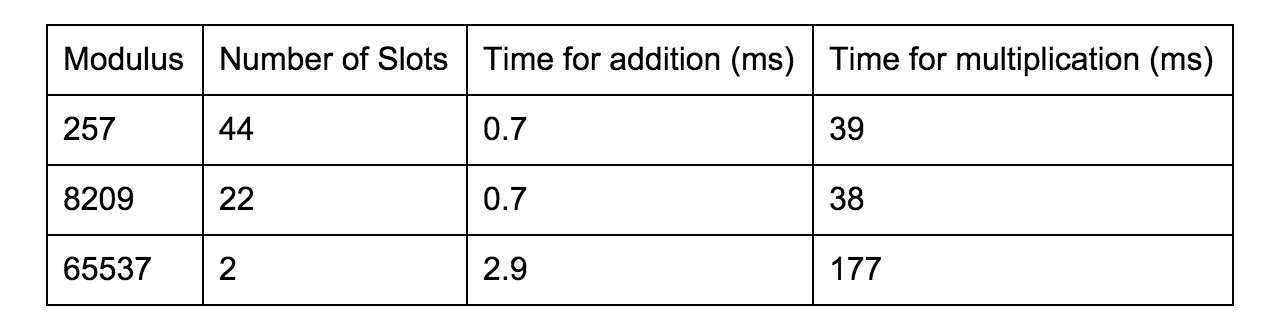
\includegraphics[width=1\textwidth]{table}
    \caption{This table shows performance of addition and multiplication based on modulus and number of slots in message. }
    \label{fig:mesh1}
\end{figure}


\section{Proof of Concept and Analysis}

To see if rendering on encrypted data is feasible, I decided to create a proof of concept by using HElib to perform a simple rendering technique called triangle rasterization. In our scenario, the ideal outcome is that a studio renders their data and the entire rendering computation can be done homomorphically in the cloud and then sent back to be decrypted. This would ensure complete security and secrecy throughout the entire process. I will describe my attempts at implementing this scenario and analyze my results. 


\subsection{Triangle Rasterization}	

The most basic rasterization algorithm takes a three-dimensional scene, described as polygons, and renders it onto a two-dimensional surface. Polygons are represented as a collection of triangles and triangles are represented by three vertices in 3D space. At a very basic level, rasterizers simply take a stream of vertices, transform them into corresponding two-dimensional points on the viewer�s monitor and fill in the transformed two-dimensional triangles as appropriate. Filling in the the transformed 2D triangles is done through the process called triangle rasterization. 

Triangle rasterization is an algorithm that takes the edge equations describing the three edges in a triangle, and after scanning all the pixels, it fills in the pixels located in the triangle. It does this through a comparison based on the pixel's x and y coordinates. 

Take for example a triangle which has the points $P_{1} (0,0)$, $P_{2} (5,0)$, and $P_{3} (0,5)$. They form the three edges $E_{1}$, $E_{2}$, $E_{3}$ where the three equations that characterize them are $y = 0$, $x=0$, and $y = -x + 5$ respectively. In the figure below you can see the points and the triangle they form. The top left pixel in the grid is at position (0,0) and x increases as you go right and y increases as you go down. Before we begin the rasterization, we modify each line equation so that they are greater or equal to zero depending on the position of the edge. Once we do this our edge inequalities are $y >= 0$, $x >= 0$, and $-x - y + 5 >= 0$. The rasterization algorithm iterates through all the pixels in the image. If a pixel's coordinates satisfy these equations, then it is colored; otherwise the nothing is done. Figure 2 shows the outcome of this rasterization. 
\begin{figure}[h!]
    \centering
        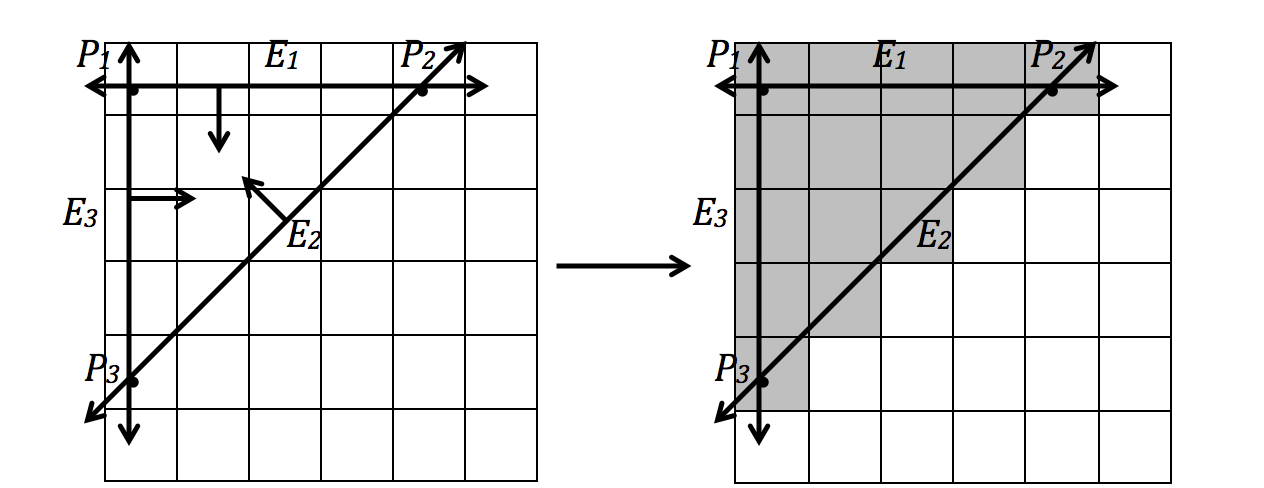
\includegraphics[width=1\textwidth]{triangle}
    \caption{Left grid shows the edges formed by points. Right grid shows result of rasterization after iterating through all pixel coordinates and coloring pixels  }
    \label{fig:mesh1}
\end{figure}

In practice, this would be done for many different triangles describing a 3D scene and each one can can be filled in with very different pixel values. In this example for simplicity I colored the pixels within the triangle grey.

\subsection{Implementation}

To create a proof of concept for rasterization on encrypted data, I implemented a triangle rasterization function in C++ utilizing HElib for encryption. The function $RASTERIZE$ takes in three sets of encrypted coefficient vectors $C_{1}$, $C_{2}$, and $C_{3}$ which describe the three edge equations for a single triangle. If we follow the same example as previously described, the three vectors of coefficients given to the function would be (0, 1, 0), (1, 0, 0), (-1, -1, 5). We encrypt these using HElib before running the function. This is because in practice, the cloud would compute this function. So to make sure all our data is secret, we encrypt it before handing the data to the cloud. As you can see from the pseudocode below, once the coefficient vectors are passed we then create the value vectors $V_{1}$, $V_{2}$, and $V_{3}$ which consist of values corresponding to each coefficient vectors and the $X$ and $Y$ vectors. The $X$ and $Y$ vectors are the encrypted x and y coordinates in the frame. So for example if the frame were to be 3x3, the $X$ vector would be (0, 1, 2, 0, 1, 2, 0, 1, 2) while the $Y$ vector would be (0, 0, 0, 1, 1, 1, 2, 2, 2). Once the value vectors are created, the algorithm iterates through the indeces of the length of the image and evaluates whether $V_{1} \geq 0$, $V_{2} \geq 0$, and $V_{3} \geq 0$. If this is the case then that pixel is colored, otherwise it is not. 

\begin{figure}[h!]
\begin{algorithmic}
\Function{$RASTERIZE$}{$C_{1}$, $C_{2}$, $C_{3}$} 
\State $V_{1} \gets X * C_{1}[0] + Y * C_{1}[1] + C_{1}[2]$
\State $V_{2} \gets X * C_{2}[0] + Y * C_{2}[1] + C_{2}[2]$
\State $V_{3} \gets X * C_{3}[0] + Y * C_{3}[1] + C_{3}[2]$ 
\For {\texttt{i in length(image)}}
\If {\texttt{$V_{1}[i]\geq 0$ AND $V_{2}[i]\geq 0$ AND $V_{3}[i]\geq 0$}}
	\State $RESULT[i]\gets 1$
\Else
	\State $RESULT[i]\gets 0$
\EndIf
\EndFor \\
\hspace{5 mm} \Return $RESULT$
\EndFunction
\end{algorithmic}
\caption{Pseudocode for triangle rasterize function  }
\end{figure}

I was able to successfully implement most of the function in C++ on encrypted data as designed. Unfortunately, HElib does not provide the functionality to perform comparisons as we need when seeing if the value vectors are greater than zero. Instead, after the value vectors are evaluated by the cloud, they are sent back to the studio, which decrypts the vectors and performs the necessary comparisons to rasterize the triangle. Thus, although not all the computations were able to be computed on encrypted data, most of the computations required by the triangle rasterization function can be computed on encrypted data homomorphically in the cloud. 


\subsection{Analysis}
The initial goal of implementing the entire triangle rasterization function encrypted was not possible because HElib does not provide a comparison operator without violating the security of the system. Nevertheless, my final implementation allows most of the operations to be done homomorphically and provides a very important proof of concept. With this implementation, a studio can send an encrypted list of coefficients describing the triangles in the frame and the cloud can compute all the vector values homomorphically. The studio can then take these results, decrypt them, and only have to perform comparisons across the pixels in the frame to render the final result. This allows studios who utilize cloud computing services to render their films to have most of their computations done homomorphically on the cloud, solving their security concerns.


\subsection{Future Work}

The future work for the project would consist of implementing the additional capability onto HElib to perform comparisons homomorphically. Since this is a very low level and complex library, adding this functionality was beyond the scope of this project, but it seems feasible after several months of research and work. There can also be a more full-scale rendering function that can be implemented to provide a more complex proof of concept for rendering on encrypted data. Furthermore, there can be testing with rendering encrypted data on an actual running cloud computing service. All this would further cement and complement the proof of concept I have provided in this paper. This is a very exciting field and as time goes on, more interesting and revolutionary implementations can be achieved.

\section{Conclusion}

This implementation of triangle rasterization with HElib forms a very powerful proof of concept of the ability to render securely. Although not all the computations were possible, the proof of concept I developed allows most of the computations to be done homomorphically and establishes a strong basis for future work. Homomorphic encryption not only can be applied in this scenario but in others as well such as such in the medical field where you can keep all of a patient's medical records  encrypted and compute on that data as well as in the financial realm when dealing with private data and functions. It can also be used to create many other secure systems, for example secure voting systems, collision-resistant hash functions, private information retrieval schemes, and many more.

This is a revolutionary field and could eventually lead to all user data to be completely secure in all systems. As interest grows and quicker schemes are being implemented, we are getting closer to this reality. This project was an important step towards showing that secure rendering is possible and other similar projects can be feasible as well.



\begin{thebibliography}{9}

\bibitem{lamport94}
  Zvika Brakerski, Craig Gentry, Vinod Vaikuntanathan
  \emph{Fully Homomorphic Encryption without Bootstrapping}
  
\bibitem{lamport94}
  Craig Gentry, Amit Sahai, Brent Waters
  \emph{Homomorphic Encryption from Learning with Errors:
Conceptually-Simpler, Asymptotically-Faster, Attribute-Based},
2013.

\bibitem{lamport94}
  Shai Halevi, Victor Shoup
  \emph{Design and Implementation of a Homomorphic-Encryption Library},
  2013.
  
  \bibitem{lamport94}
  Oded Regev,
  \emph{The Learning with Errors Problem}

\bibitem{lamport94}
  Craig Gentry,
  \emph{A FULLY HOMOMORPHIC ENCRYPTION SCHEME},
2009.

\bibitem{lamport94}
  C. Gentry, S. Halevi, N.P. Smart,
  \emph{Fully Homomorphic Encryption with Polylog Overhead},


\bibitem{lamport94}
  Kristin Lauter, Michael Naehrig, Vinod Vaikuntanathan,
  \emph{Can Homomorphic Encryption be Practical?},

\end{thebibliography}




\end{document}